\section{Experiments}

Parameter sampling for SARSA. Range sampled over $\alpha$, $\gamma$, and $\lambda$. What $\epsilon$ was used.

\subsection{Problems}
\subsubsection{Mountain Car}
\begin{figure}
\center
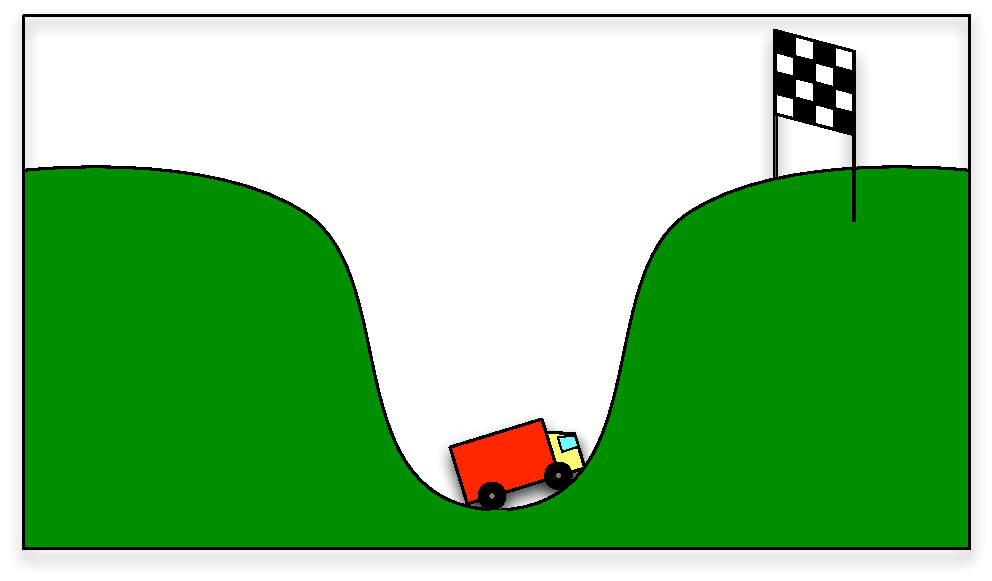
\includegraphics[width=0.75\linewidth]{MC_problem.pdf}
\caption{In the mountain car problem, a car must escape from a valey. It cannot climp the hill without moving backward first to gain speed. The agent receives a reward only when it escapes.}\label{fig:MC:problem}
\end{figure}

\subsubsection{Maze}
\begin{figure}
\center
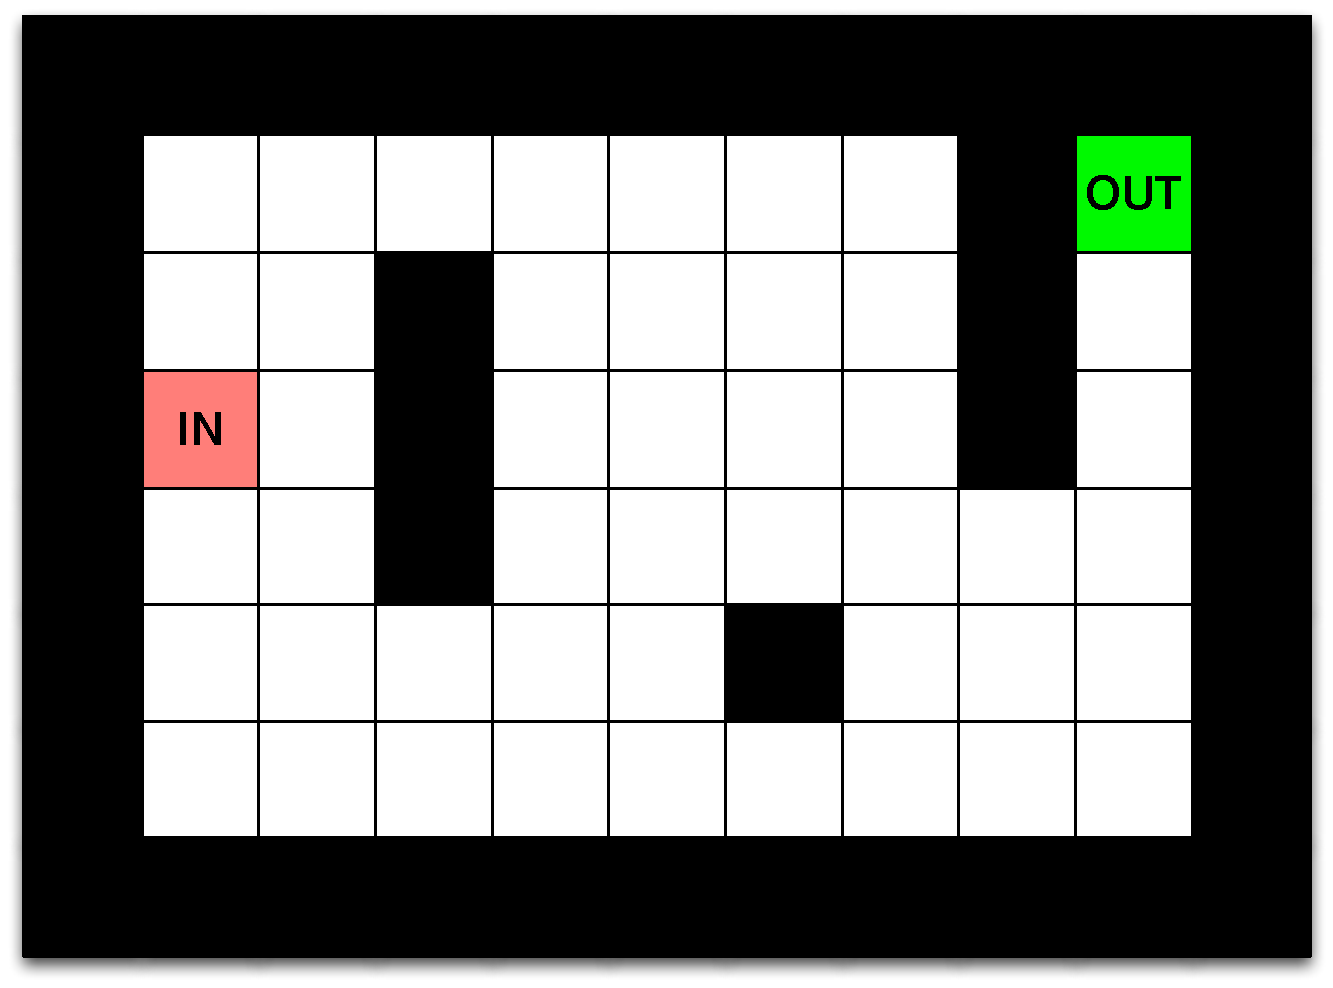
\includegraphics[width=0.75\linewidth]{MZ_problem.pdf}
\caption{In the maze problem, the agent have to find its way in a maze from the start (in red) to the end (in green). The agent receives a reward only when it escapes.}\label{fig:MC:problem}
\end{figure}

\subsubsection{Puddle World}
\begin{figure}
\center
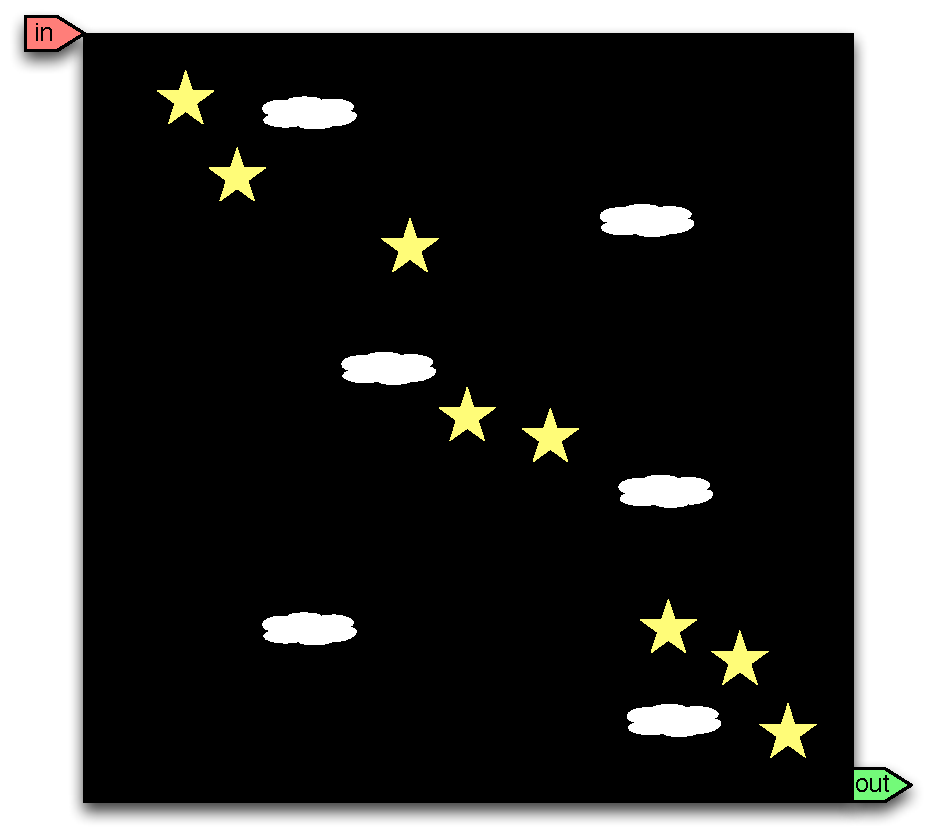
\includegraphics[width=0.75\linewidth]{PW_problem.pdf}
\caption{In the puddle world problem, the agent have to find its way in a dark environment from the start (in red) to the end (in green). Local rewards are given all along its exploration and when it escapes.}\label{fig:MC:problem}
\end{figure}

\subsubsection{Maze}

Originally introduced by Sutton as an example for deterministic problem solving with RL, maze \cite{Sutton1990}.

Evolutionary programming has previously been applied to a multi-task version of Sutton's maze problem \cite{Handa2007}.

\subsubsection{Mountain Car}

Introduced to test RL in sparse coding \cite{sutton1996generalization}

\subsubsection{Puddle World}

Stochastic

Introduced to test RL in sparse coding \cite{sutton1996generalization}

\subsubsection{Actor critic pendulum}
\begin{figure}
\center
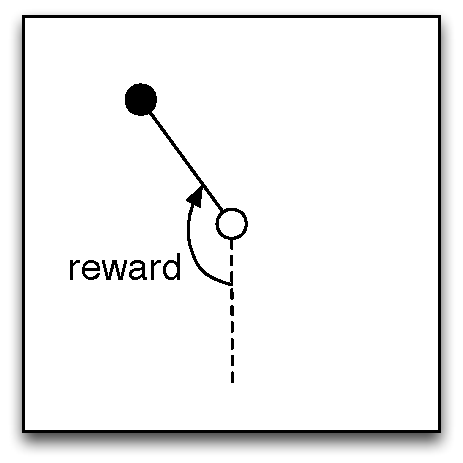
\includegraphics[width=0.5\linewidth]{ACP_problem.pdf}
\caption{In the actor critic pendulum, the agent has to balance a pendulum to the highest possible position. The reward is given by the cosinus of the angle between the pendulum and the resting position.}\label{fig:MC:problem}
\end{figure}


citation \cite{sutton1998introduction}. 

\subsection{Training GRN on one specific problem}
In this first experience, we have trained our GRN-based neuromodulation model independently on each problem above mentionned. To evaluate the gain provided by neuromodulation, we first determine the best fixed learning parameter to use with SARSA on each problem. We use parameter sampling on $\alpha$, $\gamma$ and $\lambda$ in $[0, 1]$ with 0.0714 steps (15 evaluations). Each evaluation is averaged on 10 replicates in order to reduce the randomness of the problems. At the end of the parameter sampling stage, we chose the best fixed learning parameters for a given problem by selecting the tuple with the highest fitness. These parameters are given in table \ref{tab:SARSAFixedParams}.

\begin{table}
\begin{tabular}{c|ccc}
%\cline{2-4}
					& $\alpha$	& $\gamma$	& $\lambda$	\\\hline
Mountain car			& 0.071429	& 1.0		& 0.928571 	\\%\hline
Maze				& 1.0		& 0.928571	& 0.928571	\\%\hline
Puddle world			&  0.057142	& 0.928571	& 0.5		\\%\hline
Actor critic pendulum	& 0.05		& 0.928571	& 0.785714	\\%\hline
\end{tabular}
\caption{Fixed learning parameters for SARSA obtained by parameter sampling}\label{tab:SARSAFixedParams}
\end{table}

\subsubsection{Mountain car}
First, the GRN is trained on Mountain car. Figure \ref{fig:MC:Convergence} shows the convergence curve of the genetic algorithm on this particular problem. We can observe that the best GRN is found very quickly (green curve) before being slowly optimized to regulate the learning parameters more efficiently. Figure \ref{fig:MC:GRNBehavior} plots the behavior of the best GRN obtained after 150 iterations. This figure plots the input protein concentrations and the three learning parameters calculated by the gene regulatory network. The GRN maintains the parameter values almost constant over the time except at the beginning of each episode where $\alpha$ and $\gamma$ are increase to explore more, certainly due to the novelty of the environment. In this experience, it has also to be noticed that $\lambda$ is kept to zero all over time. On this simple problem, memory might not be necessary. 

This GRN is then compared to the SARSA algorithm with fixed learning parameters on 100 independent reruns of mountain car with different different random seed. The point is to evaluate the capacity of both approaches to handle the noise generated by randomness. Figure \ref{fig:MC:GRNvsSARSA} shows the results obtained for each episode averaged on the 100 runs. We can observe that neuromodulation with GRN trained on the mountain car (in green) beats SARSA with fixed parameters (in red) on every episodes. More specifically, the first episodes (from 1 to 3) show that GRN-based neuromodulation learns faster than SARSA and later episodes (from 3 to 25) show that neuromodulation solves the problem faster than SARSA.

\begin{figure}
\center
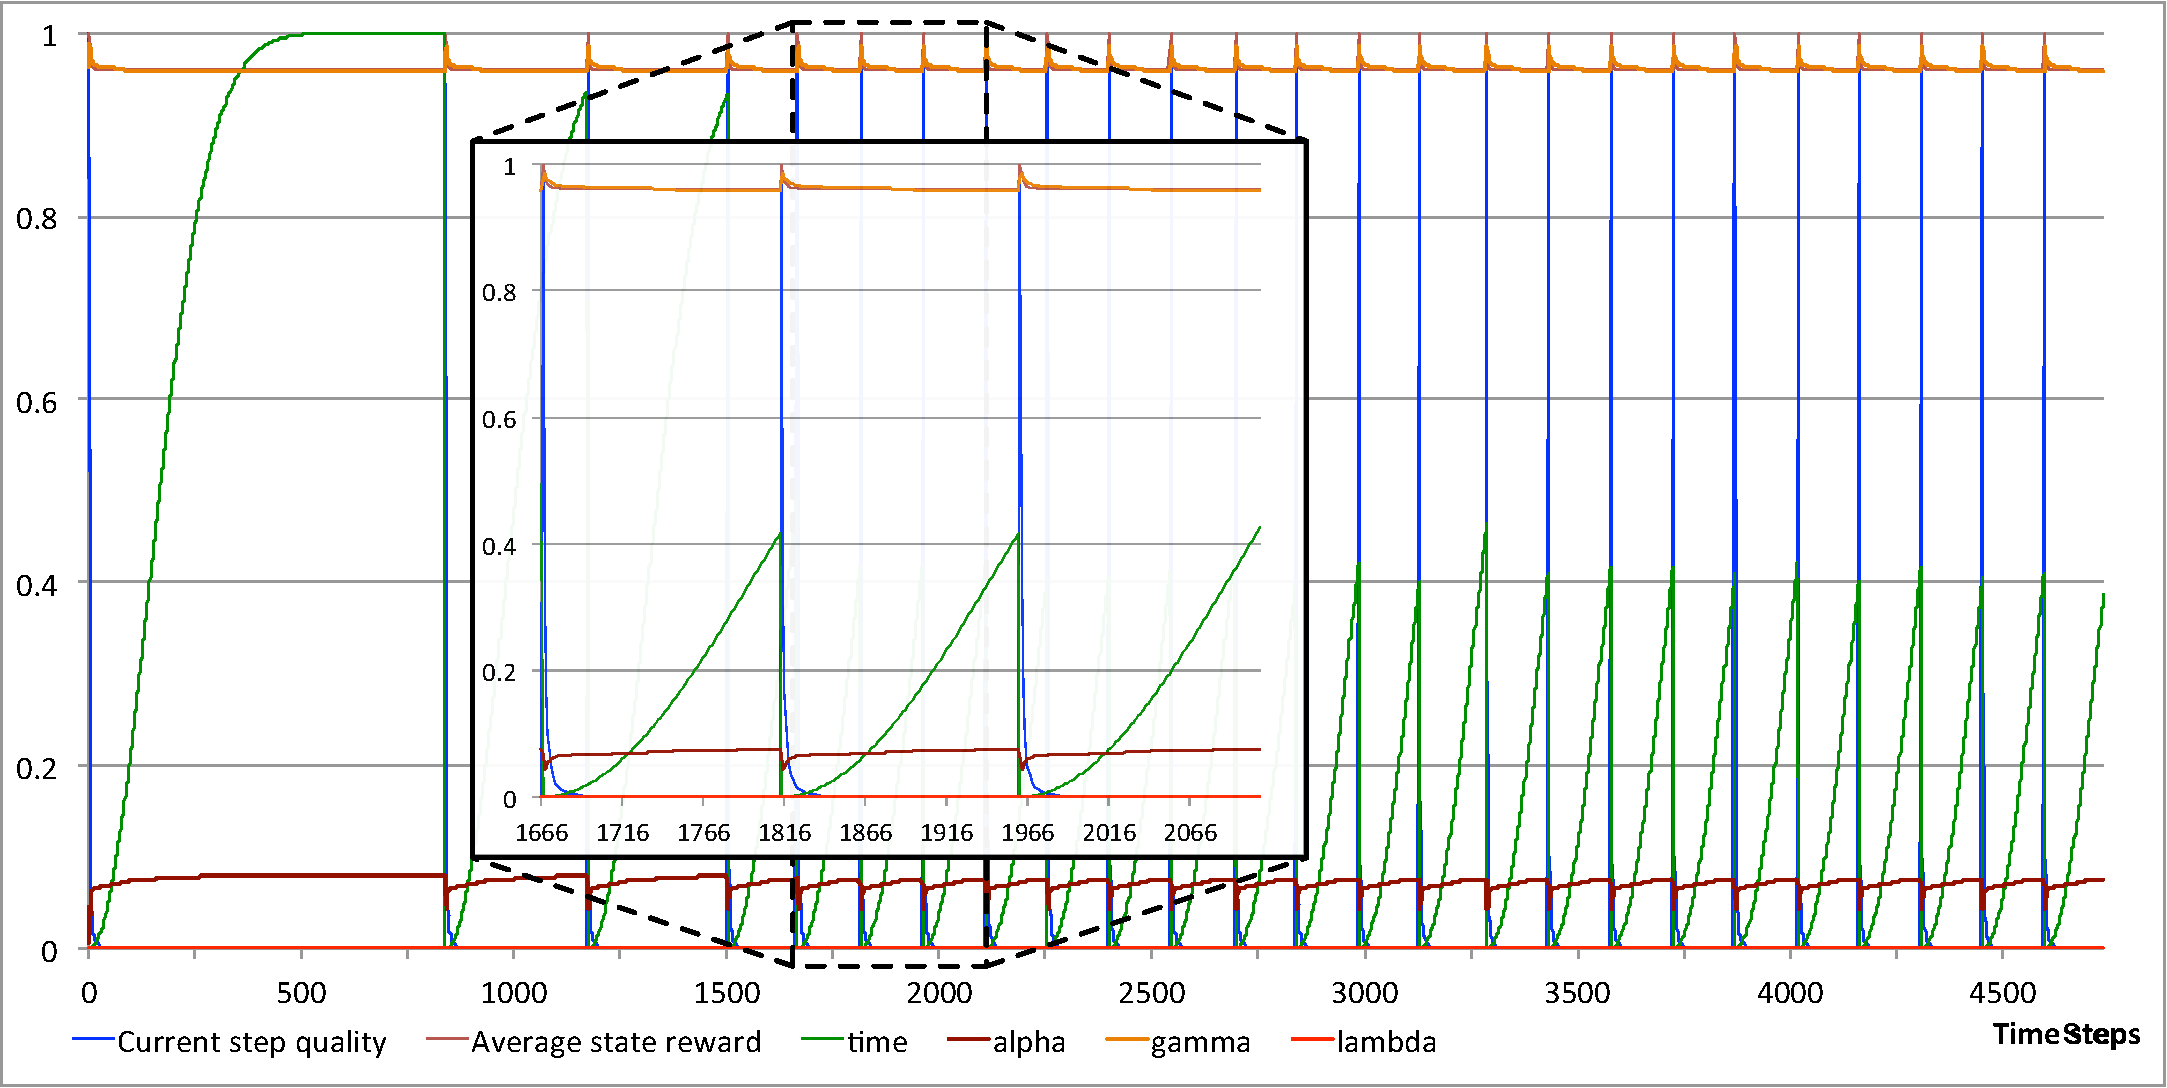
\includegraphics[width=\linewidth]{MC_GRNBehavior.pdf}
\caption{Moutain car: Regulation of the learning parameters of the best GRN obtained.}\label{fig:MC:GRNBehavior}
\end{figure}

\begin{figure}
\center
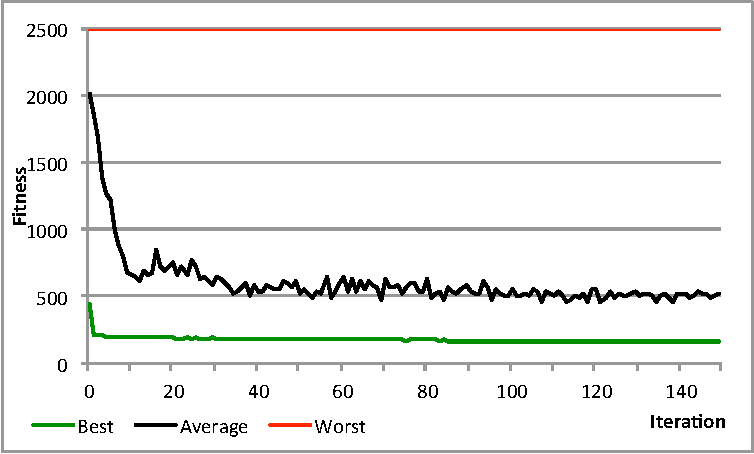
\includegraphics[width=0.75\linewidth]{MC_convergence.pdf}
\caption{Mountain car: Convergence curve of the genetic algorithm (lower is better - time to escape the valley).}\label{fig:MC:Convergence}
\end{figure}

\begin{figure}
\center
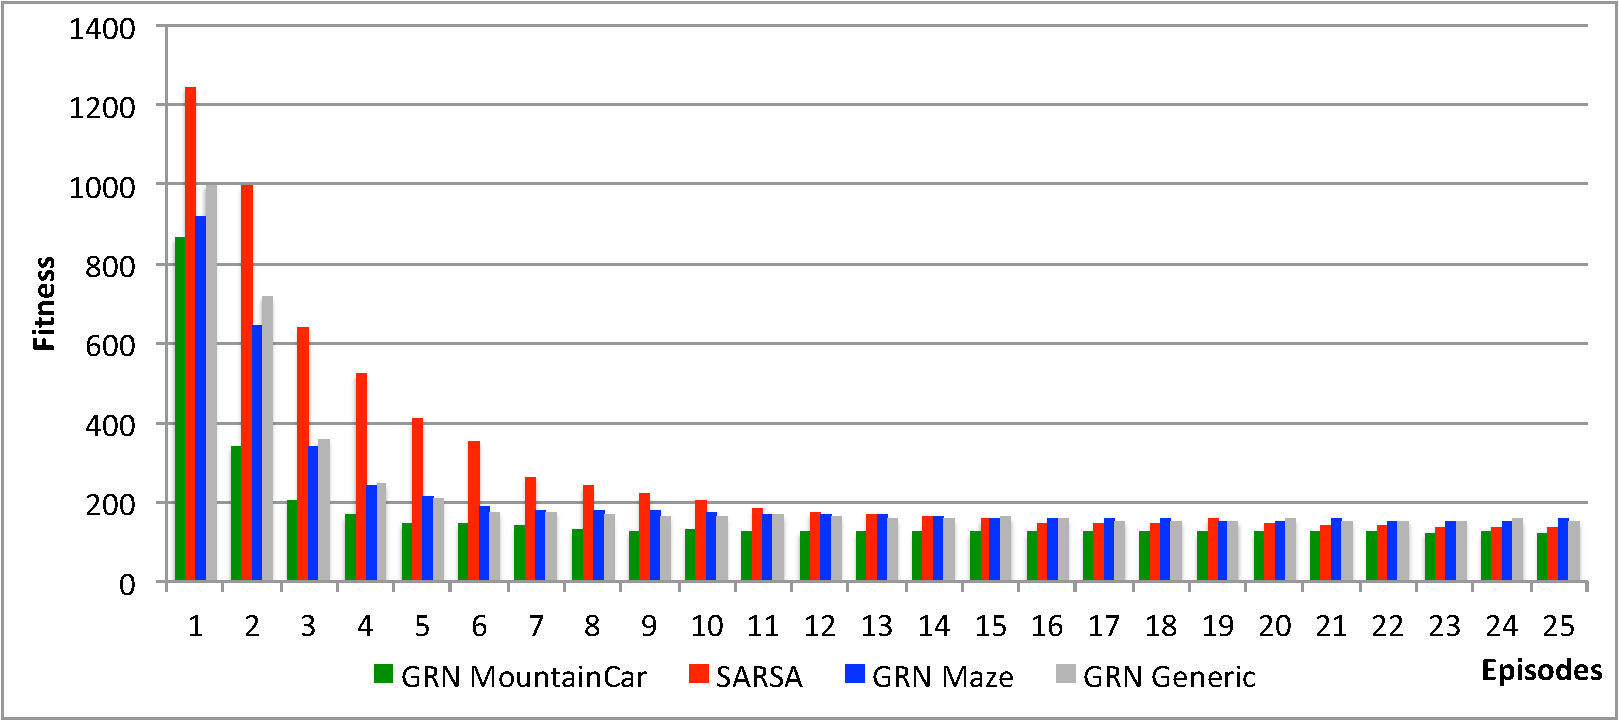
\includegraphics[width=\linewidth]{MC_GRNvsSARSA.pdf}
\caption{Mountain car: Comparison of the fitnesses per episode (abscissa) obtained by our neuromodulation with a GRN trained on mountain car (green), with a GRN trained on maze (blue) and with parameter-fixed SARSA (red). Results are averaged on 100 independent runs.}\label{fig:MC:GRNvsSARSA}
\end{figure}

\subsubsection{Maze}
The same procedure has been used to evolve a gene regulatory network to regulate SARSA's learning parameters on the maze problems. Figure \ref{fig:MZ:GRNBehavior} presents the behavior of the best GRN obtained after evolution. The regulation broadly differs from the one obtained on the mountain car problem. This GRN starts with very high values for all learning parameters with the aim to explore widely the environment. Then, with sucessfull episodes incoming, the learning rate $\alpha$ and the memory depth $\lambda$ decrease to exploit the behavior learnt during the first scenarios. $\gamma$ is kept very high all along the simulation.

When compared to parameter-fixed SARSA (figure \ref{fig:MZ:GRNvsSARSA}), we can observe that the GRN is learning faster than SARSA (episodes 2 to 5) due to its high learning rate at the begining of the simulation. However, the avantage turns to fixed-parameter SARSA in the remaining episodes: SARSA is doing slightly better than neuromodulation from episode 6 to the end.

\begin{figure}
\center
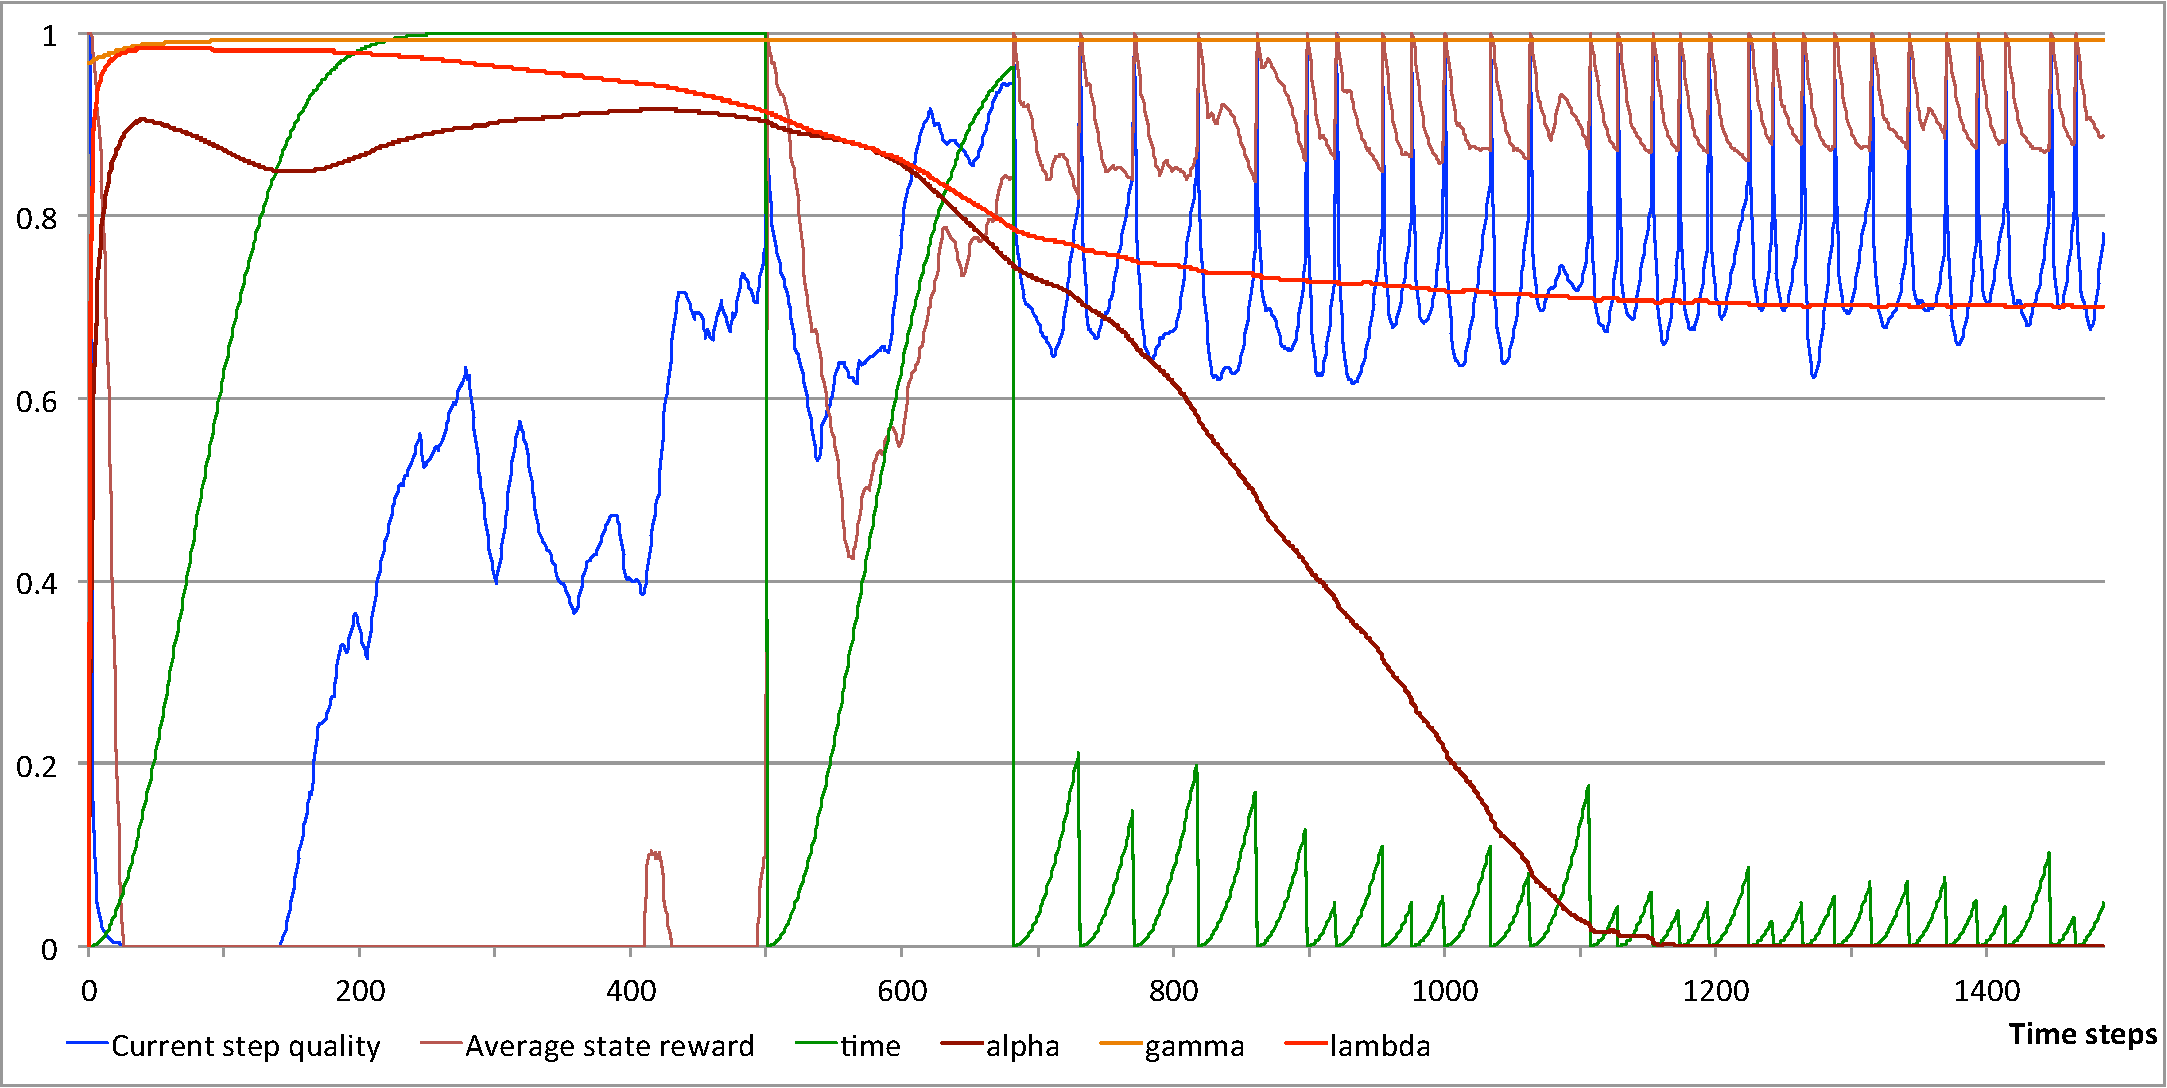
\includegraphics[width=\linewidth]{MZ_GRNBehavior.pdf}
\caption{Maze: Regulation of the learning parameters of the besst GRN obtained.}\label{fig:MZ:GRNBehavior}
\end{figure}

\begin{figure}
\center
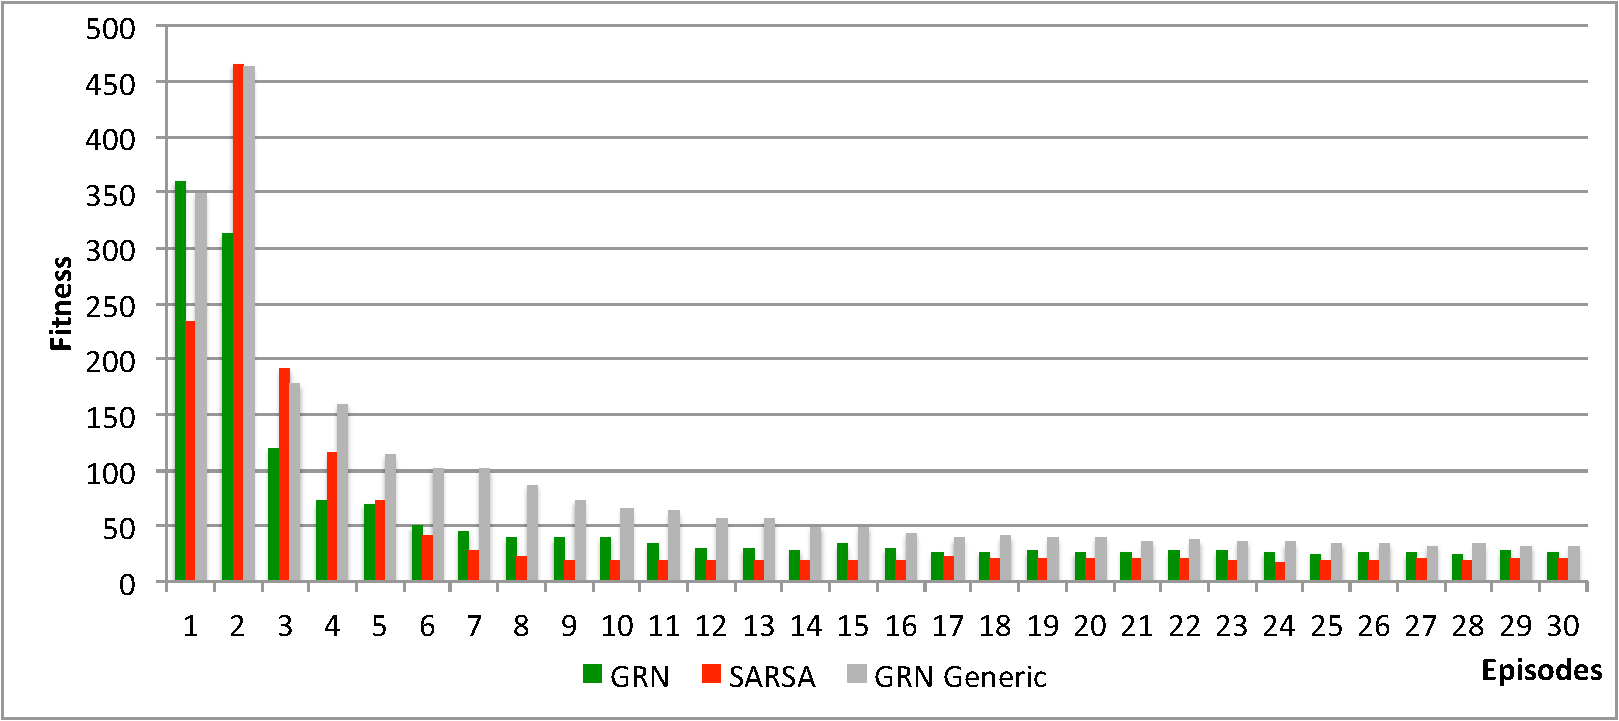
\includegraphics[width=\linewidth]{MZ_GRNvsSARSA.pdf}
\caption{Maze: Comparison of the fitnesses per episode (abscissa) obtained by our neuromodulation with a GRN trained on maze (green) and with parameter-fixed SARSA (red). Results are averaged on 100 independent runs.}\label{fig:MC:GRNvsSARSA}
\end{figure}


\subsubsection{Puddle world}

\subsubsection{Actor critic pendulum}

Number of GRN runs, number of generations

\subsection{Generalization of the regulation}

Generalizing from which problems to which other problems. Does training on stochastic and testing on deterministic lead to better GRNs than training on
deterministic then testing on stochastic?
